%%%%%%%%%%%%%%%%%%%%%%%%%%%%%%%%%%%%%%%%%%%%%%%%%%%%%%%%%%%%%%%%%%%%%
%
% An introductory course for machine learning, EEIA Godomey 2022 version
% (Rodolphe Le Riche)
%
%%%%%%%%%%%%%%%%%%%%%%%%%%%%%%%%%%%%%%%%%%%%%%%%%%%%%%%%%%%%%%%%%%%%%

\documentclass[12pt]{beamer}
\usepackage[utf8]{inputenc}
\usepackage{amsmath}
\usepackage{amsfonts}
\usepackage{amssymb}
\usepackage{graphicx}
\graphicspath{{figures/}}
%\usepackage{beamerthemesplit}
%\usepackage{beamerthemeshadow} 
\usepackage{color}
\usepackage{hyperref}
\usepackage{xspace}
\usepackage{xifthen}
\usepackage{multicol}
\usepackage{mathtools}
\usepackage{algorithm,algorithmic}
\usepackage{dsfont}
%
% these 2 next needed for mathbb greek letters
\usepackage{breqn} 
\usepackage[bbgreekl]{mathbbol}
%
\usepackage{bbm} % this one is needed for the indicator
%
\usepackage{tikz}
\usetikzlibrary{calc,shapes,arrows,positioning}
%
% handwritten font
\newcommand*{\hwfont}{\fontfamily{qzc}\selectfont}
\DeclareTextFontCommand{\texthw}{\hwfont}

% custom commands in sty file, for easier writting and change of notations
\usepackage{my_notations}

\usetheme{Madrid}
\usecolortheme{beaver}

%%%%%%%%%%%%%%%%%%%%%%%%%%%%%%%%%%%%%%%%%%%%%%%%%%%%%%%%%%%%%%%%%%%%%
\begin{document}
\title
[~Optimization for machine learning
%\hspace{0.5cm}
%\insertframenumber/\inserttotalframenumber
]
{An introduction to optimization for machine learning}
\author
[Le Riche et al.]
{\large Rodolphe Le Riche$^1$, Dédji Brian Whannou$^2$, Kévin Kpakpo Akouété$^3$} 
\institute[CNRS/fondat. Vallet]{
$^1$ CNRS LIMOS at Mines Saint-Etienne, France \\
$^2$ UBS Group AG \\
$^3$ Descartes Underwriting
} 
\date[July 2022]{July 2022 \\
Ecole d'Eté en Intelligence Artificielle \\
fondation Vallet\\
Cotonou, Bénin} 
\begin{frame}
\titlepage
\end{frame}

\section{Introduction}
\subsection{Objectives, acknowledgements}

%%%%%%%%%%%%%%%%%%%%%%%%%%%%%%%%%%%%%%%%%%%%%%%%%%%%%%%%%%%%%%%%%
\begin{frame}
\frametitle{Foreword}
This course was given during a summer school on AI in Godomey, Benin, July-Aug. 2022.
The school was organized by the Benin Excellence NGO and the Vallet Foundation (cf. 
{\scriptsize
\url{https://www.fondationvallet.org/eeia}}
).
\begin{itemize}
\item The course provides basic concepts for numerical optimization
\item for an audience interested in machine learning
\item with a background corresponding to 1 year after high school
\item through examples coded in python from scratch.
\item Limitation: the algorithms are not exactly those used in state-of-the-art deep learning, but the main concepts, related to gradient descent, will be presented.
\end{itemize}
The code, the slides and the project statement are available at {\scriptsize \url{https://github.com/rleriche/Optimization_AI_Cotonou_2022}}
\end{frame}

%%%%%%%%%%%%%%%%%%%%%%%%%%%%%%%%%%%%%%%%%%%%%%%%%%%%%%%%%%%%%%%%%%
\begin{frame}%[allowframebreaks]
\frametitle{Course outline} 
\begin{multicols}{2}
\begin{center} \textbf{An introduction to optimization for machine learning} \end{center}
\tableofcontents[currentsection]
\end{multicols}
\end{frame}

%%%%%%%%%%%%%%%%%%%%%%%%%%%%%%%%%%%%%%%%%%%%%%%%%%%%%%%%%%%%%%%%%
\begin{frame}
\frametitle{Bibliographical references for the class}
{\small
This course is based on
\begin{itemize}
\item \cite{ravikumar17} : a detailed up-to-date presentation of the main convex optimization algorithms for machine learning (level end of undergraduate, bac +3)
\item \cite{minoux2008programmation} : a classic textbook for optimization, written before the ML trend but still useful (level end of undergraduate / bac+3)
\item \cite{bishop2006pattern} : a reference book for machine learning with some pages on optimization (level end of undergraduate / bac+3)
\item \cite{schmidt2007fast} : L1 regularization techniques (research article)
\item \cite{sun2019optimization} : review of optimization methods and good practices for tuning neural nets.
\end{itemize}
The content of these references will be simplified for this class.
} % end small font
\end{frame}

\subsection{Optimization problem formulation}

%%%%%%%%%%%%%%%%%%%%%%%%%%%%%%%%%%%%%%%%%%%%%%%%%%%%%%%%%%%%%%%%%
\begin{frame}
\frametitle{Optimization = a quantitative formulation of decision}
Optimization is a\footnote{non unique, incomplete when considering human beings or life} way of mathematically modeling decision.
\vskip\baselineskip
\mbox{
\begin{minipage}[c]{0.3\textwidth}

\includegraphics[width=\textwidth]{decision-clipart.jpg}
\end{minipage}
\begin{minipage}[c]{0.7\textwidth}
\begin{equation*}
\min_{x \in \mathcal S} f(x)
\end{equation*}
\begin{itemize}
\item $x$ vector of decision parameters (variables)~: dimensions, investment, tuning of a machine / program, \ldots
\item $f(x)$~: decision cost $x$
\item $\mathcal S$~: set of possible values for $x$, search space
\end{itemize}
\end{minipage}
} % end mbox
\end{frame}

%%%%%%%%%%%%%%%%%%%%%%%%%%%%%%%%%%%%%%%%%%%%%%%%%%%%%%%%%%%%%%%%%
\begin{frame}
\frametitle{Optimization example: design}
\begin{center}
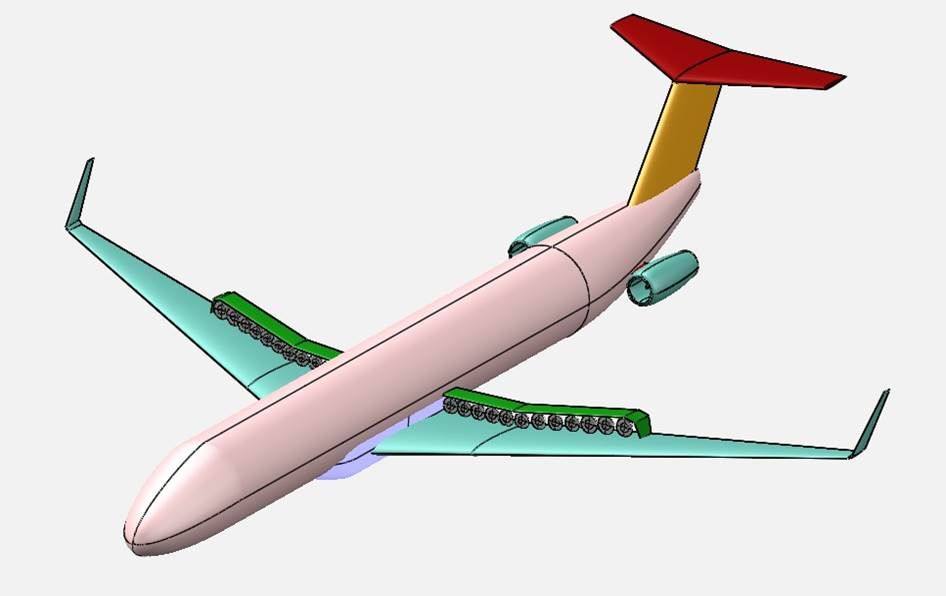
\includegraphics[width=0.5\textwidth]{aircraft_distributed_prop.png}\\
\vspace{-1cm}
{\hfill\tiny (from \cite{sgueglia2018exploration})}
\end{center}
\vskip\baselineskip
$x$ = aircraft parameters (here distributed electrical propulsion)\\
$f()$ = $-1\times$ performance metric (aggregation of $-1\times$ range, cost, take-off length, \ldots) \\
At the minimum, the design is ``optimal''.
\end{frame}

%%%%%%%%%%%%%%%%%%%%%%%%%%%%%%%%%%%%%%%%%%%%%%%%%%%%%%%%%%%%%%%%%
\begin{frame}
\frametitle{Optimization example: model identification}
\begin{center}
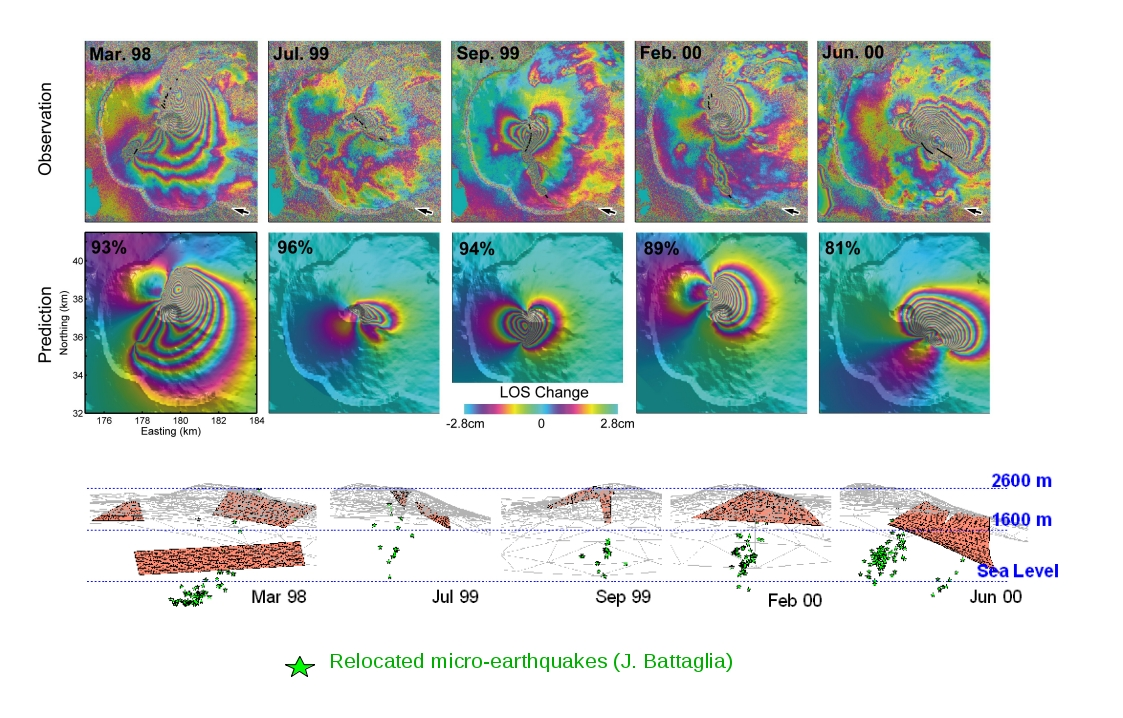
\includegraphics[width=0.7\textwidth]{piton_fournaise.jpg}\\
\vspace{-1cm}
{\hfill\tiny (from \cite{fukushima2010evolution})}
\end{center}
$x$ = dike position, geometry, internal pressure\\
$f()$ = distance between measures (from RADARSAT-1 satellite) and model (boundary elements, non trivial computation)\\
At the minimum, the model best matches measurements and should correspond to the underground phenomenon.
\end{frame}


\subsection{Examples of optimization usages}

%%%%%%%%%%%%%%%%%%%%%%%%%%%%%%%%%%%%%%%%%%%%%%%%%%%%%%%%%%%%%%%%%
\begin{frame}
\frametitle{Optimization example: neural net classification}
\vspace{-0.3cm}
Predict if a person stays at home or goes out based on longitude, latitude and temperature = a 2 classes classification problem.
\begin{center}
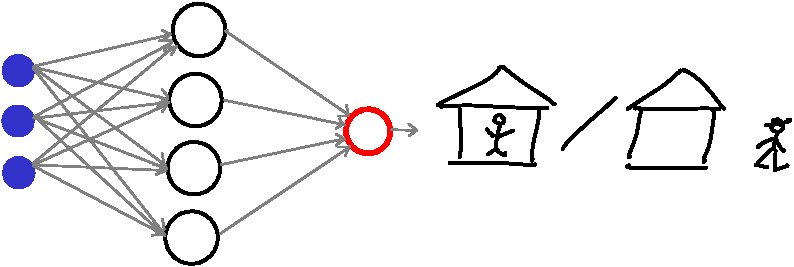
\includegraphics[width=0.6\textwidth]{neuralnet3-4-1-classif-crop.pdf}\\
\vspace{-0.5cm}
\end{center}
$x$ = neural network (NN) weights and biases\\
$f()$ = an error of the NN predictions (a cross-entropy error):
\begin{itemize}
\item $e$ entries: $e_1$ longitude, $e_2$ latitude, $e_3$ temperature
\item $t=1$ if person stays, $t=0$ otherwise
\item Observed data set: $(e^i,t^i),~ i=1,\ldots,N$
\item $y(e;x)$: output of the NN, the probability that $t(e)=1$ 
\item $f(x) = - \sum_{i=1}^N \{ t^i \log(y(e^i;x)) + (1-t^i) \log(1 - y(e^i;x))\}$
\end{itemize}
\end{frame}

%%%%%%%%%%%%%%%%%%%%%%%%%%%%%%%%%%%%%%%%%%%%%%%%%%%%%%%%%%%%%%%%%
\begin{frame}
\frametitle{\small (a word on the classification cross-entropy error)}
\begin{itemize}
\item View the relationship between the entry $e$ and the class $t$ as probabilistic (generalizes deterministic functions): $t(e)$ is a Bernoulli variable with a given probability that $t(e)=1$
\item The NN models this probability: $y(e;x)$ is the probability that $t(e)=1$, $1-y(e;x)$ is the proba that $t(e)=0$, $0\le y(e;x) \le 1$.
\item The probability of $t$ knowing $e$ can be written $y(e;x)^{t}\times(1-y(e;x))^{1-t}$
\item The likelihood of the $N$ i.i.d observations is $\prod_{i=1}^N \left[y(e^i;x)^{t^i}\times(1-y(e^i;x))^{1-t^i}\right]$, to be maximized
\item The likelihood is turned into an error, to be minimized, by taking $-\log(\text{likelihood})$, 
\begin{equation*}
f(x) = - \sum_{i=1}^N \{ t^i \log(y(e^i;x)) + (1-t^i) \log(1 - y(e^i;x))\}
\end{equation*}
\end{itemize}
\end{frame}

%%%%%%%%%%%%%%%%%%%%%%%%%%%%%%%%%%%%%%%%%%%%%%%%%%%%%%%%%%%%%%%%%
\begin{frame}
\frametitle{Optimization example: neural net regression}
\vspace{-0.3cm}
learn a function from a discrete limited set of observations
%\begin{center}
%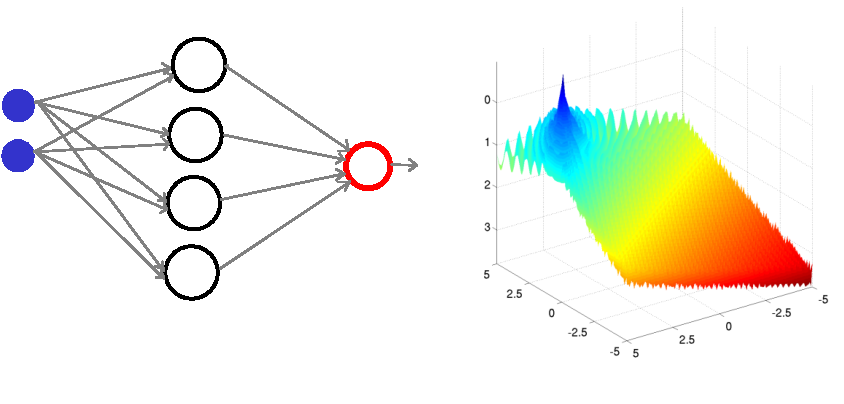
\includegraphics[width=0.6\textwidth]{neuralnet3-4-1-regress-crop.pdf}\\
%\vspace{-0.5cm}
%\end{center}
\begin{center}
\begin{minipage}{0.6\textwidth}
\begin{tikzpicture}
\node[anchor=south west,inner sep=0, outer sep=0] (contour) at (0,0) {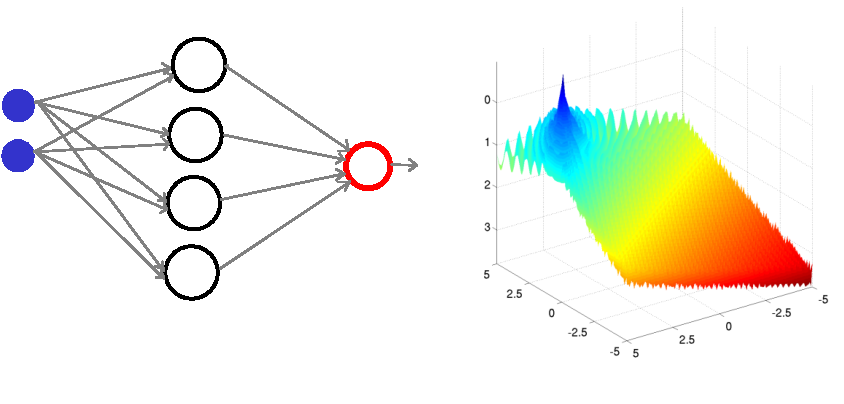
\includegraphics[width=\textwidth]{neuralnet3-4-1-regress-crop.pdf}};
\begin{scope}[x={(contour.south east)},y={(contour.north west)}]
%\draw[help lines,xstep=0.1,ystep=0.1] (0,0) grid (1,1);
\node[] (e1) at (0.6,0.2) {\small $e_1$};
\node[] (e2) at (0.9,0.15) {\small $e_2$};
\node[] (t) at (0.6,0.85) {\small $t(e)$};
\node[] (e1NN) at (-0.05,0.75) {\small $e_1$};
\node[] (e2NN) at (-0.05,0.60) {\small $e_2$};
\node[] (yy) at (0.48,0.69) {\small $y(e \mathchar\numexpr"6000+`;\relax x)$};
\draw[black,fill=black] (0.6,0.63) circle (.15ex);
\draw[black,fill=black] (0.9,0.35) circle (.15ex);
\draw[black,fill=black] (0.665,0.78) circle (.15ex);
\draw[black,fill=black] (0.78,0.7) circle (.15ex);
\draw[black,fill=black] (0.7,0.5) circle (.15ex);
\draw[black,fill=black] (0.85,0.55) circle (.15ex);
\draw[black,fill=black] (0.75,0.35) circle (.15ex);
\end{scope}
\end{tikzpicture}
\end{minipage}
\end{center}
\vspace{-0.5cm}
$x$ = neural network (NN) weights and biases\\
$f()$ = an error of the NN predictions (sum-of-squares error):
\begin{itemize}
\item $e$ entries, $t(e)$ target function to learn
\item observed data set, ``\tikz\draw[black,fill=black] (0,0) circle (.15ex);'' : $(e^i,t^i),~ i=1,\ldots,N$
\item $y(e;x)$: output of the NN, the expected value of $t(e)$ 
\item $f(x) = 1/2 \sum_{i=1}^N (t^i - y(e^i;x))^2 $
\end{itemize}
\end{frame}

%%%%%%%%%%%%%%%%%%%%%%%%%%%%%%%%%%%%%%%%%%%%%%%%%%%%%%%%%%%%%%%%%
\begin{frame}
\frametitle{Optimization example: image denoising}
\vspace{-0.5cm}
\begin{equation*}
\begin{split}
\min_x f(x) \quad,\quad & f(x) = \frac{1}{2}\sum_{i=1}^{N_{\text{pixels}}} (y_i - x_i)^2 + 
\lambda \sum_{i=1}^{N_{\text{pixels}}} \sum_{j \text{ near } i} \lvert x_i - x_j \rvert \\
& \lambda \ge 0 \quad\text{regularization constant}
\end{split}
\end{equation*}
\begin{center}
\begin{minipage}[t]{0.2\textwidth}

\includegraphics[width=\textwidth]{c_clean.png} \\
{\small target image}
\end{minipage}
\hfill
\begin{minipage}[t]{0.2\textwidth}
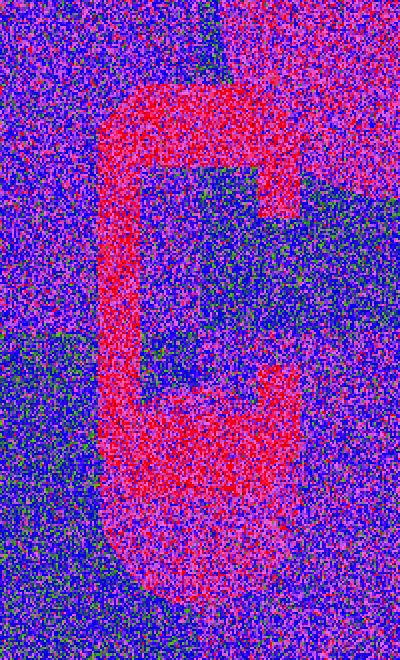
\includegraphics[width=\textwidth]{c_noisy.png} \\
{\small \mbox{noisy (observed)} $= y_i$'s}
\end{minipage}
\hfill
\begin{minipage}[t]{0.2\textwidth}
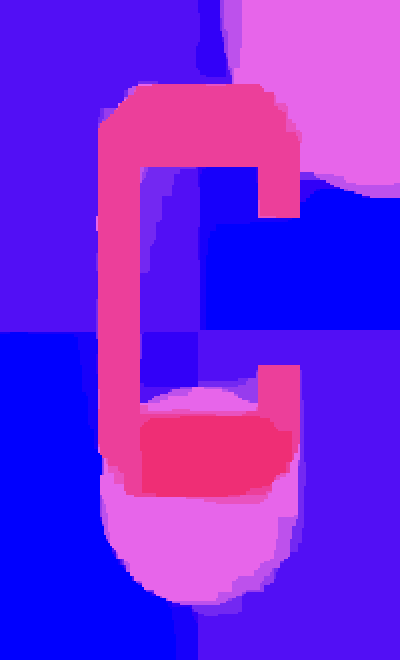
\includegraphics[width=\textwidth]{c_denoised.png} \\
{\small \mbox{denoised (optimized)} $=x^\star$}
\end{minipage}
\mbox{\quad}
\end{center}
{\scriptsize (from \cite{ravikumar17}) \hfill}
\end{frame}


\subsection{Basic mathematical concepts for optimization}

%%%%%%%%%%%%%%%%%%%%%%%%%%%%%%%%%%%%%%%%%%%%%%%%%%%%%%%%%%%%%%%%%%
\begin{frame}%[allowframebreaks]
\frametitle{Basic mathematical concepts for optimization} 
\begin{multicols}{2}
\tableofcontents[currentsection]
\end{multicols}
\end{frame}

%%%%%%%%%%%%%%%%%%%%%%%%%%%%%%%%%%%%%%%%%%%%%%%%%%%%%%%%%%%%%%%%%%
\begin{frame}
\frametitle{Local versus global optimum} 
\vspace{-0.5cm}
\begin{equation*}
\min_{x \in \mathcal S \subset \Rset[n]} f(x)
\end{equation*}
\vspace{-0.5cm}
\begin{center}
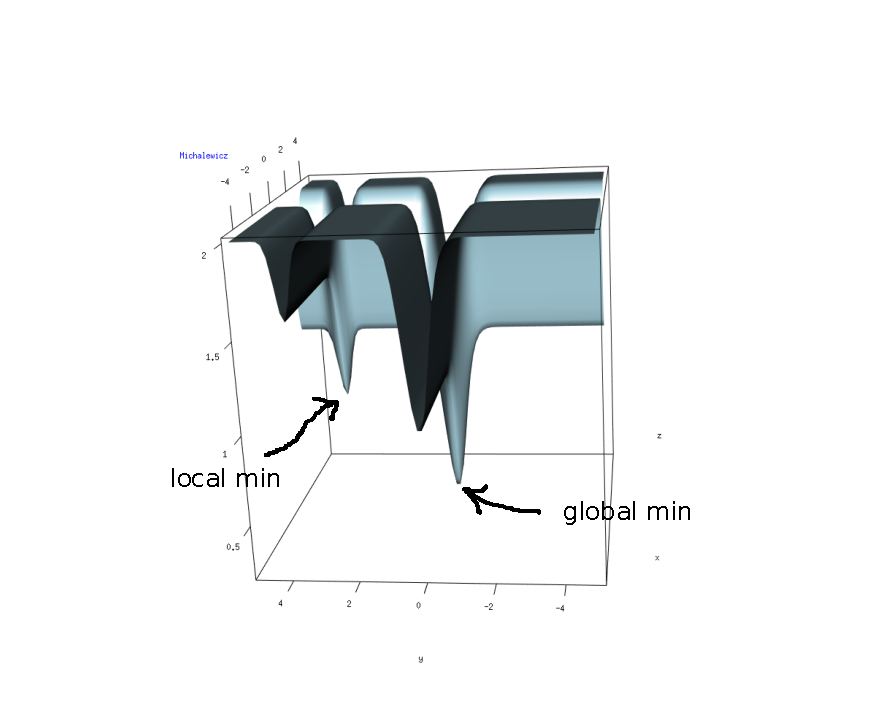
\includegraphics[width=0.7\textwidth]{michalewicz_function_annotated-crop.pdf} \\
\end{center}
\vspace{-1.0cm}
Python code to generate such a 3D plot given in the \texttt{Code} folder, \texttt{3D\_plots.py} \\
\vfill
\end{frame}

%%%%%%%%%%%%%%%%%%%%%%%%%%%%%%%%%%%%%%%%%%%%%%%%%%%%%%%%%%%%%%%%%%
\begin{frame}
\frametitle{Gradient of a function} 
Gradient of a function = direction of steepest ascent = vector of partial derivatives
\begin{equation*}
\grad f(x) = \begin{pmatrix} \frac{\partial f}{\partial x_1}(x) \\ \ldots \\ \frac{\partial f}{\partial x_n}(x) \end{pmatrix}
\end{equation*}
\begin{center}
\begin{minipage}[t]{0.7\textwidth}
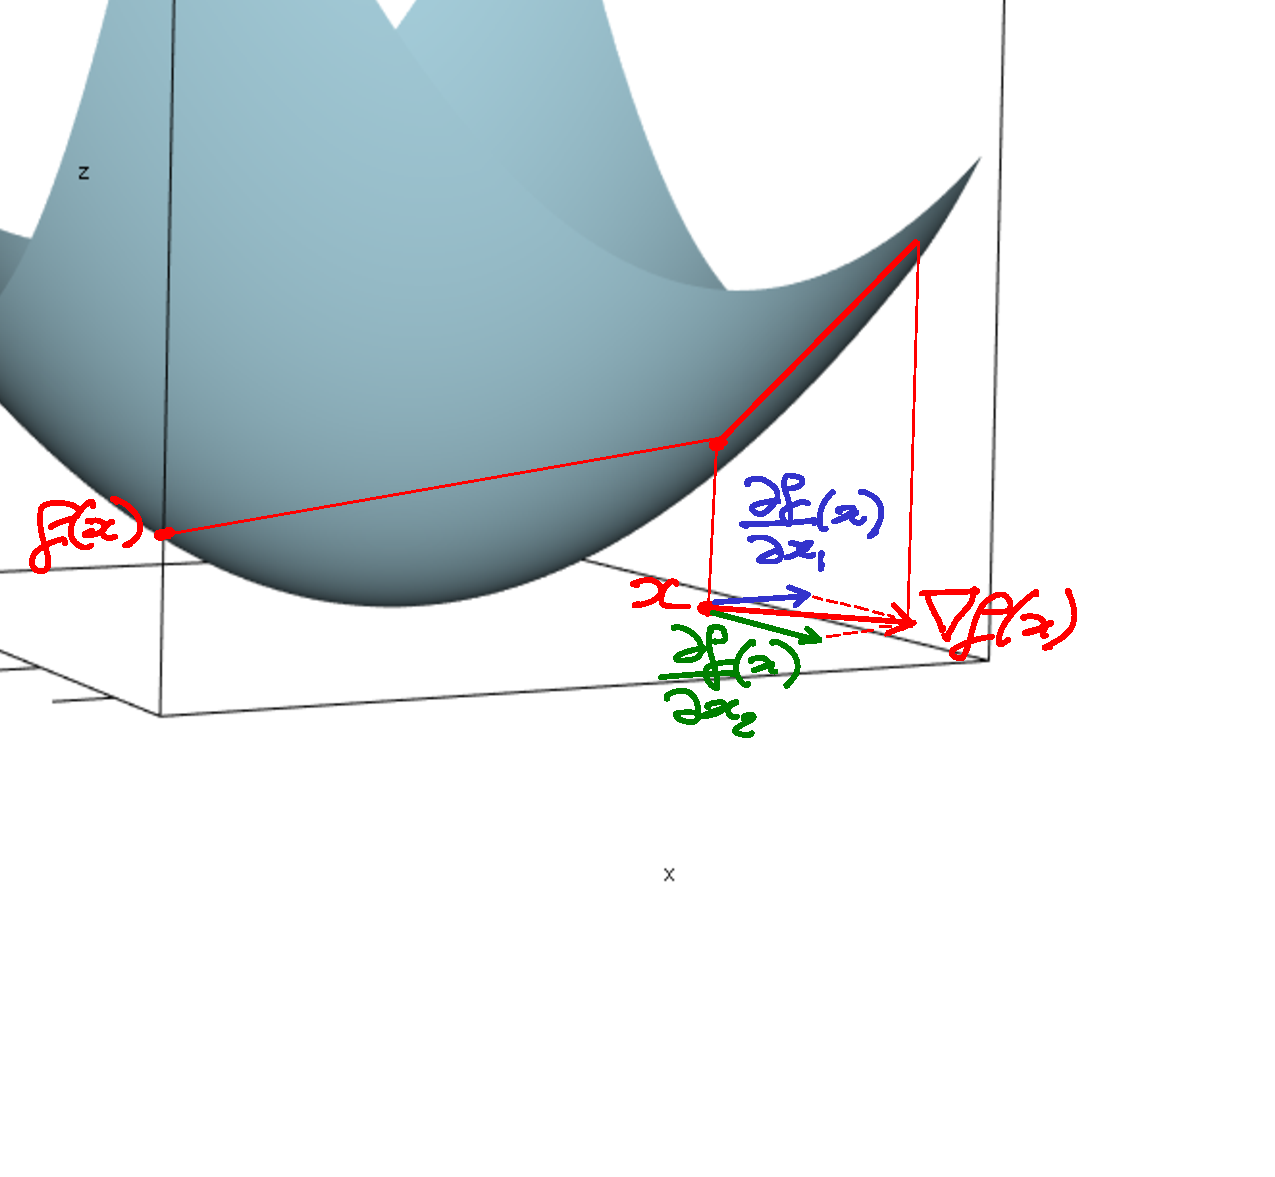
\includegraphics[width=\textwidth]{gradient-crop.pdf} \\
\end{minipage}
\end{center}
\end{frame}

%%%%%%%%%%%%%%%%%%%%%%%%%%%%%%%%%%%%%%%%%%%%%%%%%%%%%%%%%%%%%%%%%%
\begin{frame}
\frametitle{Hessian of a function} 
It is the matrix of second derivatives, 
\begin{equation*}
\hess f(x) = 
\begin{bmatrix}
\frac{\partial^2 f(x)}{\partial x_1^2} & \frac{\partial^2 f(x)}{\partial x_1 \partial x_2} & \ldots & \frac{\partial^2 f(x)}{\partial x_1 \partial x_n}\\ 
\frac{\partial^2 f(x)}{\partial x_1 \partial x_2} & \frac{\partial^2 f(x)}{\partial x_2^2} & \ldots & \frac{\partial^2 f(x)}{\partial x_2 \partial x_n}\\
\ldots & \ldots & \ddots & \ldots \\
\frac{\partial^2 f(x)}{\partial x_1 \partial x_n} & \frac{\partial^2 f(x)}{\partial x_2 \partial x_n} & \ldots & \frac{\partial^2 f(x)}{\partial x_n^2}
\end{bmatrix}
\end{equation*}
= the matrix of curvatures = the gradient of the gradient.
\end{frame}

%%%%%%%%%%%%%%%%%%%%%%%%%%%%%%%%%%%%%%%%%%%%%%%%%%%%%%%%%%%%%%%%%%
\begin{frame}[allowframebreaks]
\frametitle{Quadratic function and Hessian} 
\vskip -0.5cm
\begin{equation*}
f(x) ~=~ \frac{1}{2} x^\top H x \quad , \quad \hess f(x) = H
\end{equation*}
a good approximation to what happens on any function when converging
\mbox{
\begin{minipage}{0.5\textwidth}
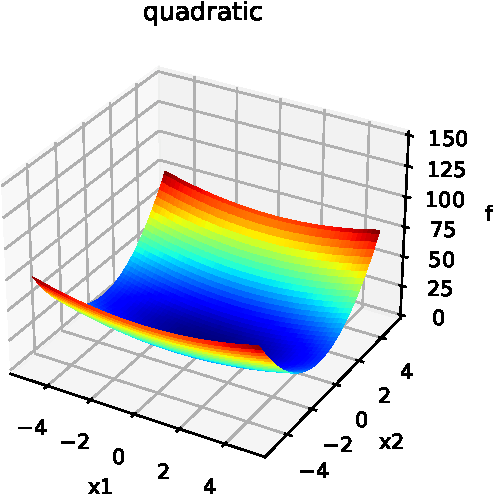
\includegraphics[width=\textwidth]{quad_rot0_cond5_H_1_0_0_5-crop.pdf}
\end{minipage}
\begin{minipage}{0.4\textwidth}
\begin{equation*}
H = \begin{bmatrix} 1 & 0 \\ 0 & 5\end{bmatrix}
\end{equation*}
\vskip\baselineskip
(guess the eigenvalues and eigenvectors)
\end{minipage}
}
%%%
\newpage
\begin{minipage}{0.5\textwidth}
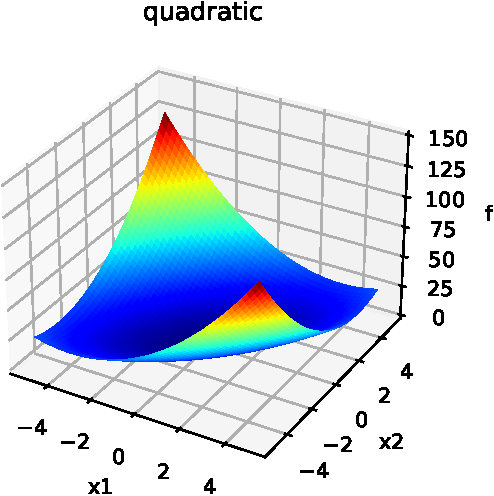
\includegraphics[width=\textwidth]{quad_rot45_cond5_H_3_m2_m2_3-crop.pdf}
\end{minipage}
\begin{minipage}{0.4\textwidth}
the same rotated by 45$^\circ$
\begin{align*}
H =& \begin{bmatrix} 3 & -2 \\ -2 & 3\end{bmatrix}  \\
\text{eig.vect} =& \begin{bmatrix} \sqrt{2}/2 & -\sqrt{2}/2 \\  \sqrt{2}/2 & \sqrt{2}/2 \end{bmatrix}\\
\text{eig.val} = & [1, 5]
\end{align*}
\end{minipage}
%%%
\newpage
\begin{minipage}{0.5\textwidth}
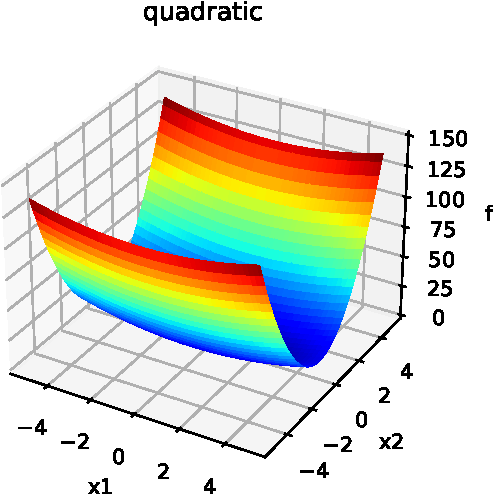
\includegraphics[width=\textwidth]{quad_rot0_cond10_H_1_0_0_10-crop.pdf}
\end{minipage}
\begin{minipage}{0.4\textwidth}
increased curvature \\ 
(condition number)
\begin{align*}
H =& \begin{bmatrix} 1 & 0 \\ 0 & 10\end{bmatrix}  
\end{align*}
\end{minipage}
%%%
\newpage
\begin{minipage}{0.5\textwidth}
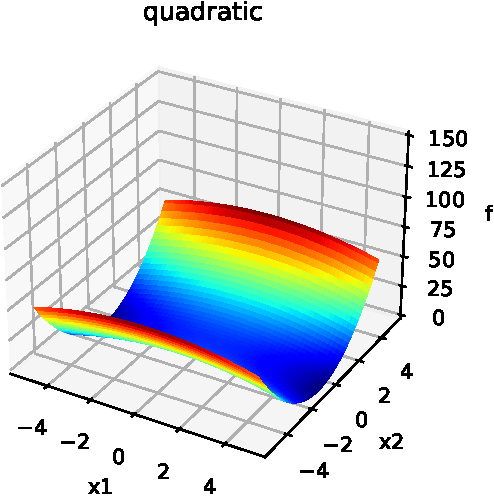
\includegraphics[width=\textwidth]{quad_rot0_condm5_H_m1_0_0_5-crop.pdf}
\end{minipage}
\begin{minipage}{0.4\textwidth}
Non positive definite Hessian
\begin{align*}
H =& \begin{bmatrix} -1 & 0 \\ 0 & 5\end{bmatrix}  
\end{align*}
what is the problem ?
\end{minipage}
\end{frame}

%%%%%%%%%%%%%%%%%%%%%%%%%%%%%%%%%%%%%%%%%%%%%%%%%%%%%%%%%%%%%%%%%%
\begin{frame}
\frametitle{Numerical approximation of the gradient} 
\mbox{
\begin{minipage}[b]{0.6\textwidth}
By forward finite differences 
\begin{equation*}
\frac{\partial f(x)}{\partial x_i} \approx \frac{f(x+h e^i)-f(x)}{h}
\end{equation*}
{Proof: \scriptsize
 by Taylor,\\
$f(x+he^i) = f(x) + h {e^i}^\top . \grad f(x) + h^2/2 {e^i}^\top \hess f(x+\rho h e^i) e^i~,~\rho\in ]0,1[$ \\
$\partial f(x)/\partial x_i = \frac{f(x+he^i)-f(x)}{h} - h/2 {e^i}^\top \hess f(x+\rho h e^i) e^i $ \\
and make $h$ very small $\square$
}
\end{minipage}
\begin{minipage}[b]{0.4\textwidth}
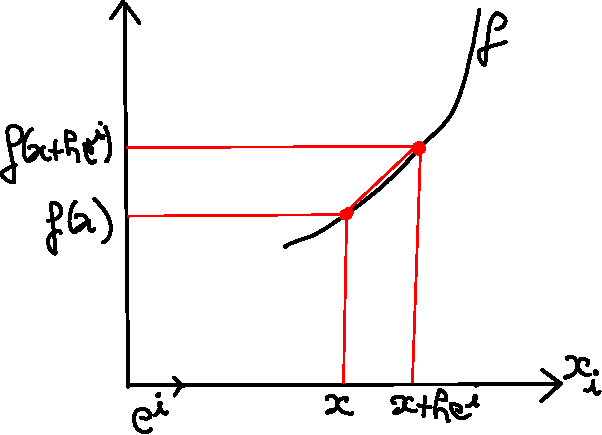
\includegraphics[width=\textwidth]{finitediff-crop.pdf}
\end{minipage}
} % mbox
\vskip\baselineskip
Other (better but more difficult to implement) schemes: central differences, automatic differentiation (e.g., in TensorFlow or PyTorch), (semi-)analytic differentiation (e.g., backpropagation in NN).
\end{frame}

%%%%%%%%%%%%%%%%%%%%%%%%%%%%%%%%%%%%%%%%%%%%%%%%%%%%%%%%%%%%%%%%%%
\begin{frame}
\frametitle{Descent direction} 
\mbox{
\begin{minipage}[b]{0.5\textwidth}
A search direction $d$ which makes an acute angle with $-\grad f(x)$ is a descent direction, i.e., for a small enough step, $f$ is guaranteed to decrease!
\end{minipage}
\hfill
\begin{minipage}[t]{0.4\textwidth}
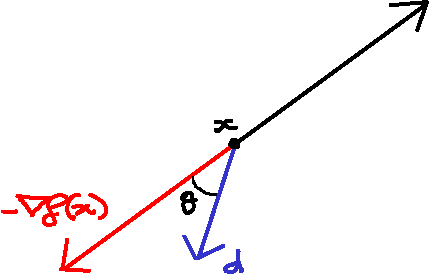
\includegraphics[width=\textwidth]{descent_direction-crop.pdf}
\end{minipage}
}
\\\vspace{0.8cm}
{\normalsize
Proof: by Taylor, $\forall \alpha,~\exists \epsilon \in [0,1]$ such that
$f(x+\alpha d) = f(x) + \alpha d^\top . \grad f(x) + \frac{\alpha^2}{2} d^\top \hess f(x + \alpha \epsilon d) d$\\
$\lim_{\alpha \rightarrow 0^+} \frac{f(x+\alpha d) - f(x)}{\alpha} = d^\top . \grad f(x) = - 1\times \lVert \grad f(x)\rVert \cos(d,-\grad f(x))$ \\
is negative if the cosine is positive $\square$
} %end small
\end{frame}

%%%%%%%%%%%%%%%%%%%%%%%%%%%%%%%%%%%%%%%%%%%%%%%%%%%%%%%%%%%%%%%%%%
\begin{frame}
\frametitle{Necessary optimality condition (1)} 
A necessary condition for a differentiable function to have a minimum at $x^\star$ is that it is flat at this point, i.e., its gradient is null
\begin{equation*}
x^\star \in \arg \min_{x \in \mathcal S} f(x) \Rightarrow \grad f(x^\star) = 0
\end{equation*}
\vskip\baselineskip
\begin{center}
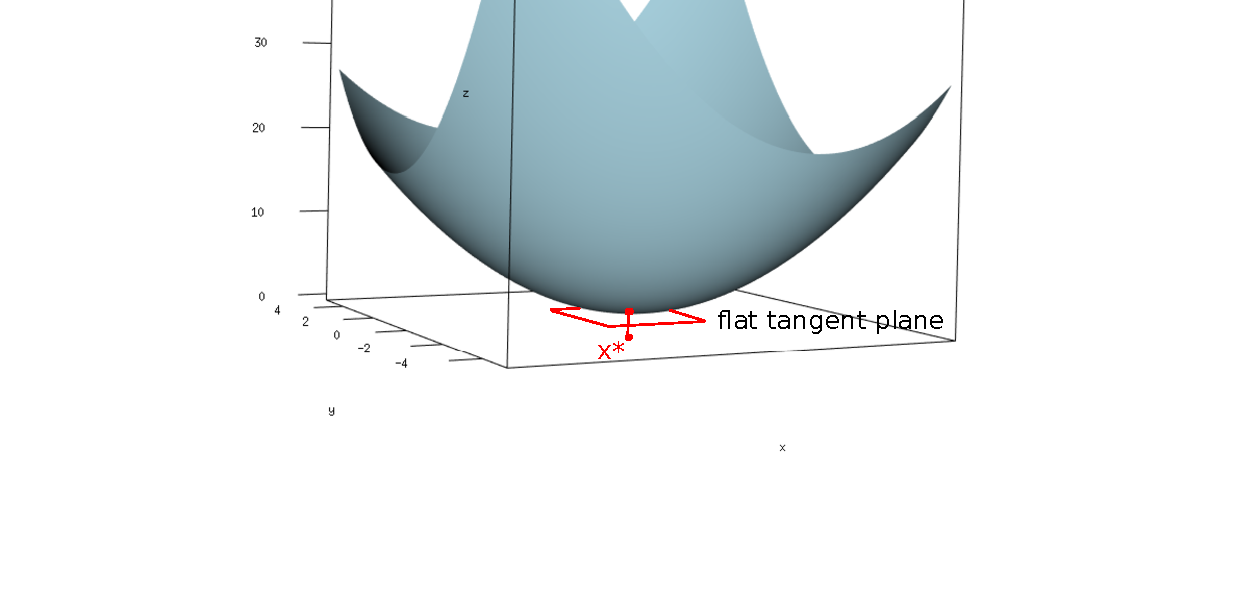
\includegraphics[width=1.2\textwidth]{minimum-crop.pdf} \\
\end{center}
\end{frame}

%%%%%%%%%%%%%%%%%%%%%%%%%%%%%%%%%%%%%%%%%%%%%%%%%%%%%%%%%%%%%%%%%%
\begin{frame}
\frametitle{Necessary optimality condition (2)} 
\begin{center}
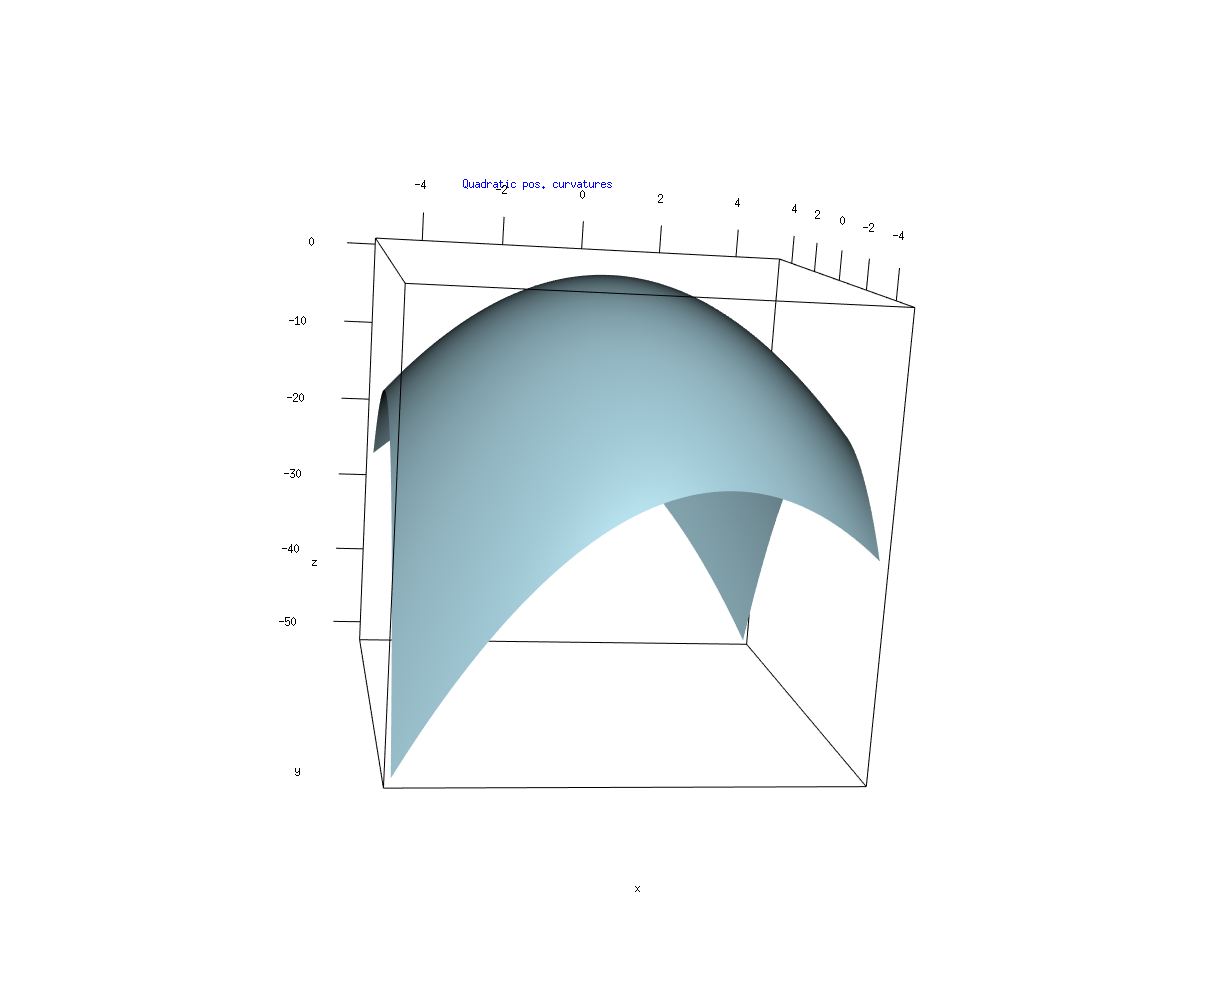
\includegraphics[width=0.7\textwidth]{quad_neg_curv.png} \\
necessary is not sufficient (works with a max) 
\vspace{2cm}
\end{center}
\end{frame}

%%%%%%%%%%%%%%%%%%%%%%%%%%%%%%%%%%%%%%%%%%%%%%%%%%%%%%%%%%%%%%%%%%
\begin{frame}
\frametitle{Necessary optimality condition (3)} 
\begin{center}
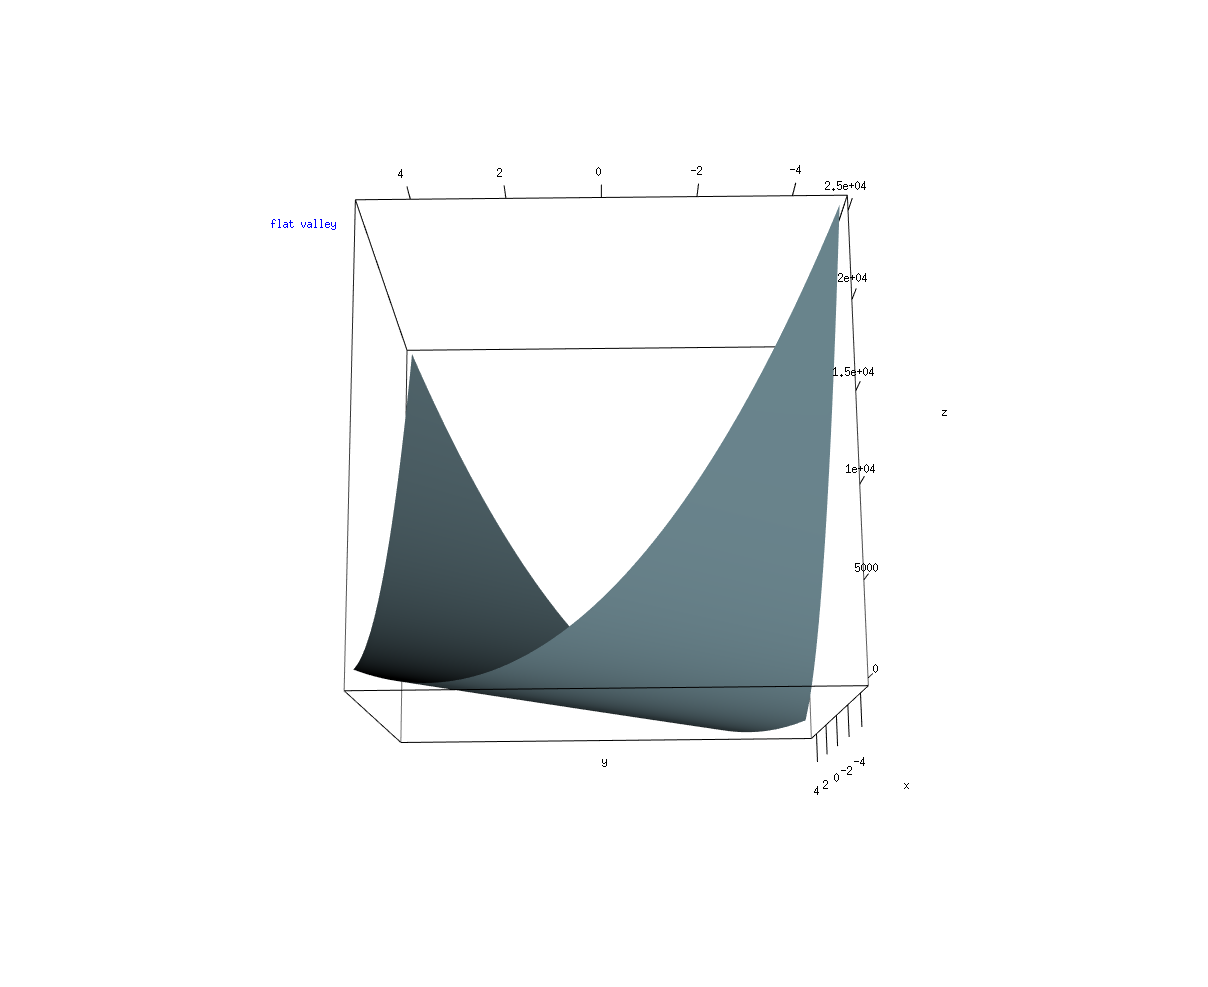
\includegraphics[width=0.7\textwidth]{flat_valley.png} \\
$\grad f(x^\star) = 0$ does not make $x^\star$ unique (flat valley)
\end{center}
\end{frame}

%%%%%%%%%%%%%%%%%%%%%%%%%%%%%%%%%%%%%%%%%%%%%%%%%%%%%%%%%%%%%%%%%%
\begin{frame}
\frametitle{Necessary optimality condition (4)} 
\begin{center}
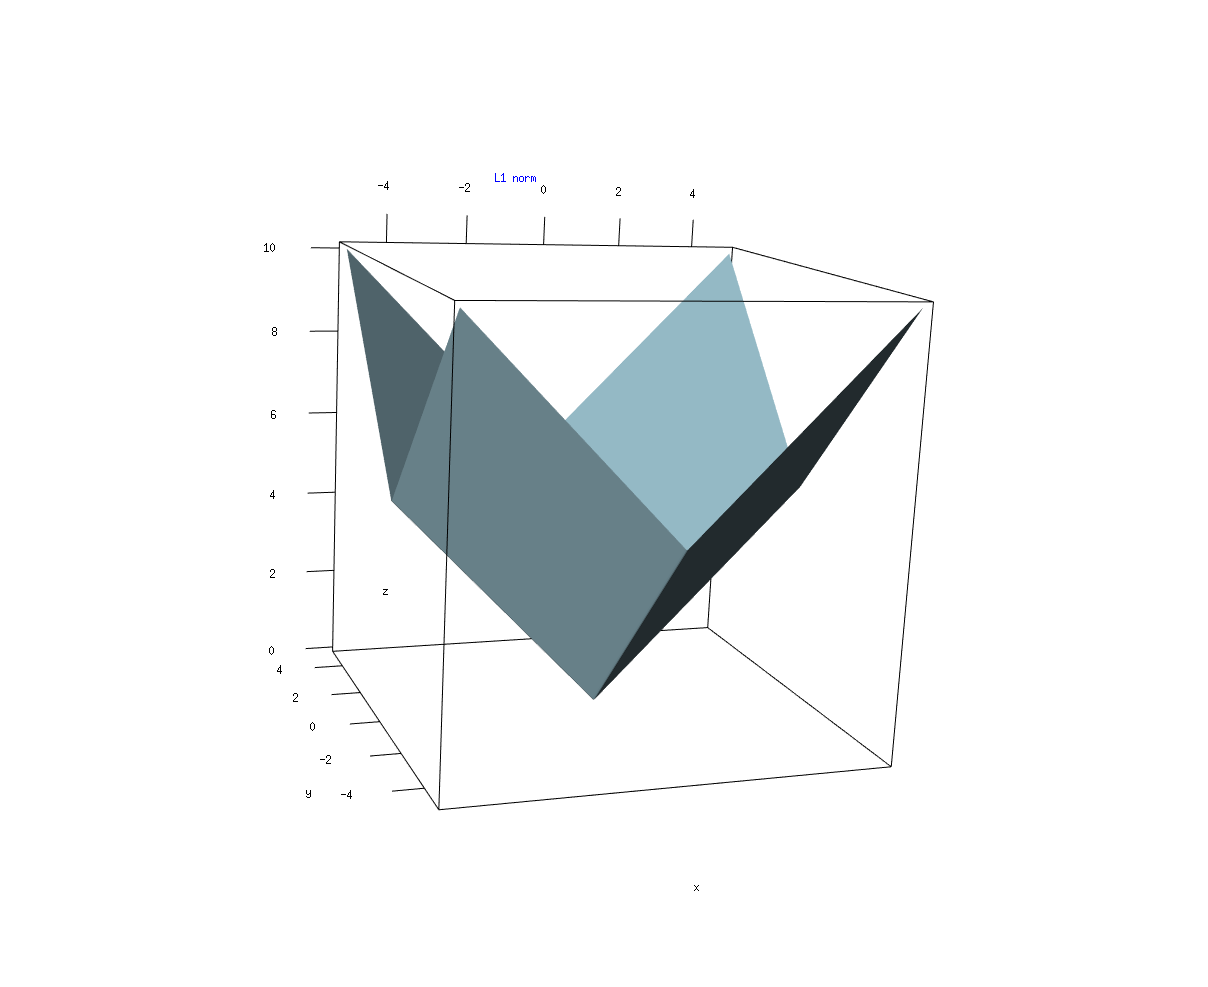
\includegraphics[width=0.7\textwidth]{L1norm.png} \\
$\grad f()$ not defined everywhere, example with L1 norm $= \sum_i^n \lvert x_i \rvert$
\end{center}
\end{frame}


\section{Steepest descent algorithm}

%%%%%%%%%%%%%%%%%%%%%%%%%%%%%%%%%%%%%%%%%%%%%%%%%%%%%%%%%%%%%%%%%%
\begin{frame}%[allowframebreaks]
\frametitle{Course outline} 
\begin{multicols}{2}
\begin{center} \textbf{An introduction to optimization for machine learning} \end{center}
\tableofcontents[currentsection]
\end{multicols}
\end{frame}


%%%%%%%%%%%%%%%%%%%%%%%%%%%%%%%%%%%%%%%%%%%%%%%%%%%%%%%%%%%%%%%%%%
\begin{frame}
\frametitle{Optimizers as iterative algorithms} 
\begin{equation*}
\text{We look for }\quad  x^\star \in \arg\min_{x \in \mathcal S} f(x) \quad,\quad \mathcal S = \Rset[n]
\end{equation*}
\begin{itemize}
\item Except for special cases (e.g., convex quadratic problems), the solution is not obtained analytically through the optimality conditions ($\grad f(x^\star) = 0$ + higher order conditions). 
\item We typically use iterative algorithms: $x^{i+1}$ depends on previous iterates, $x^1,\ldots,x^i$ and their $f$'s.
\item Often calculating $f(x^i)$ takes more computation than the optimization algorithm itself.
\item Qualities of an optimizer: robustness, speed of convergence. Have to strike a compromise between them.
\end{itemize}
\end{frame}

\subsection{Fixed step steepest descent algorithm}

%%%%%%%%%%%%%%%%%%%%%%%%%%%%%%%%%%%%%%%%%%%%%%%%%%%%%%%%%%%%%%%%%%
\begin{frame}
\frametitle{Fixed step steepest descent algorithm (1)} 
Repeat steps along the steepest descent direction, $-\grad f(x^t)$ \cite{cauchy1847methode,curry1944method}. \\
The size of the steps is proportional to the gradient norm.
\begin{block}{}
\begin{algorithmic}
\REQUIRE $f()$, $\bar\alpha \in ]0,1]$, $x^1$, $\epsilon^{\text{step}}$, $\epsilon^{\text{grad}}$, $i^{\text{max}}$
\STATE $i\leftarrow 0$, $f^{\text{bestSoFar}} \leftarrow $ \texttt{max\_double}
\REPEAT 
\STATE $i \leftarrow i+1$
\STATE calculate $f(x^i)$ and $\grad f(x^i)$
\IF{$f(x^i)< f^{\text{bestSoFar}}$} 
\STATE update $x^{\text{bestSoFar}}$ and $f^{\text{bestSoFar}}$ with current iterate
\ENDIF
\STATE \textbf{direction: } $d^i = - \grad f(x^i) / \lVert \grad f(x^i) \rVert$
\STATE \textbf{step: } $x^{i+1} ~=~ x^i + \bar\alpha \lVert \grad f(x^i) \rVert d^i$
\UNTIL{ {$i>i^{\text{max}}$} \OR {$\lVert x^i - x^{i-1}\rVert \le \epsilon^{\text{step}}$} \OR {$\lVert \grad f(x^i)\rVert/\sqrt{n} \le \epsilon^{\text{grad}}$} }
\RETURN $x^{\text{bestSoFar}}$ and $f^{\text{bestSoFar}}$
\end{algorithmic}
\end{block}
\end{frame}

%%%%%%%%%%%%%%%%%%%%%%%%%%%%%%%%%%%%%%%%%%%%%%%%%%%%%%%%%%%%%%%%%%
\begin{frame}
\frametitle{(code organization)} 
\begin{itemize}
\item \texttt{main\_optim.py}: main script for starting the descent algorithms.
\item \texttt{gradient\_descent.py}: gradient-based descent algorithms; the current gradient fixed-step version, and the ones coming up (other direction, with a line search).
\item \texttt{random\_search.py}: a random search algorithm.
\item \texttt{test\_functions.py}: a collection of test functions.
\item \texttt{3D\_plots.py}: plots a 2 dimensional function in a 3D dynamic plot + contour plot.
\item \texttt{optim\_utilities.py}: additional routines.
\end{itemize}
\end{frame}

%%%%%%%%%%%%%%%%%%%%%%%%%%%%%%%%%%%%%%%%%%%%%%%%%%%%%%%%%%%%%%%%%%
\begin{frame}
\frametitle{Fixed step steepest descent algorithm (2)} 
\begin{itemize}
\item The choice of the step size factor $\bar\alpha$ is critical : the steeper the function, the smaller $\bar\alpha$. Default value = 0.1
\item The true code (cf. \texttt{gradient\_descent.R}) is a bit longer because it is necessary to record the points visited.
\end{itemize}
\vspace{-0.5cm}
\begin{center}
{\scriptsize $f(x) = 1/2 x^\top H x$ , $H$ positive definite}\\
\begin{minipage}[b]{0.3\textwidth}
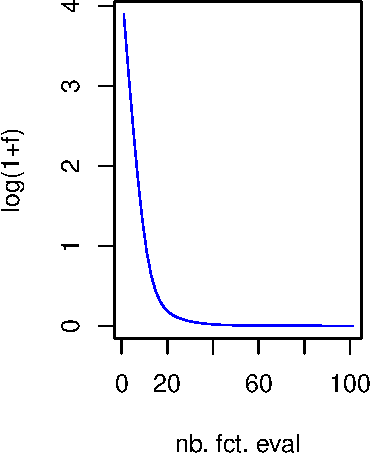
\includegraphics[width=\textwidth]{gradient_quad_2d_f_alpha01-crop.pdf} 
\end{minipage}
\hspace{1.5cm}
\begin{minipage}[b]{0.3\textwidth}
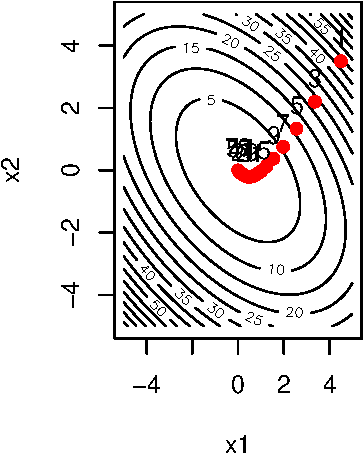
\includegraphics[width=\textwidth]{gradient_quad_2d_x_alpha01-crop.pdf} 
\end{minipage}
\end{center}
\end{frame}

%%%%%%%%%%%%%%%%%%%%%%%%%%%%%%%%%%%%%%%%%%%%%%%%%%%%%%%%%%%%%%%%%%
\begin{frame}
\frametitle{Fixed step steepest descent algorithm (3)} 
$\bar\alpha=0.1$ on $f(x)=$ Rosenbrock (banana shaped) function in $d=2$ dimensions, example of divergence:
\vskip\baselineskip
\begin{center}
\begin{minipage}[b]{0.3\textwidth}
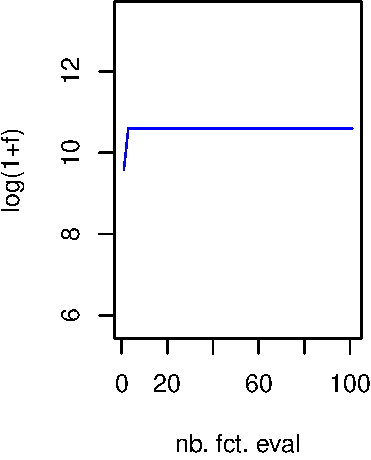
\includegraphics[width=\textwidth]{gradient_rosen_alpha0.1_f_diverges-crop.pdf} 
\end{minipage}
\hspace{1.5cm}
\begin{minipage}[b]{0.3\textwidth}
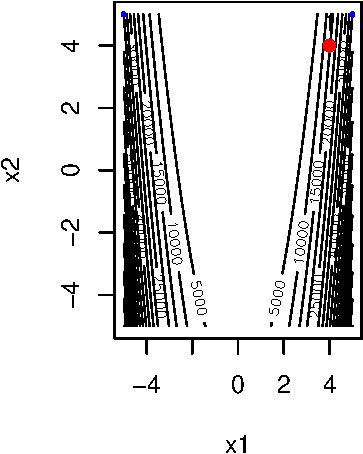
\includegraphics[width=\textwidth]{gradient_rosen_alpha0.1_x_diverges-crop.pdf} 
\end{minipage}
$x^\star = (1,1) ~,~ f(x^\star) = 0$
\end{center}
\end{frame}

\subsection{Line search}


%%%%%%%%%%%%%%%%%%%%%%%%%%%%%%%%%%%%%%%%%%%%%%%%%%%%%%%%%%%%%%%%%%
\begin{frame}
\frametitle{Descent with line search} 
\vspace{-0.5cm}
At each iteration, search for the best step size in the descent\footnote{if $d^i$ is not a descent direction, $-d^i$ is. Proof left as exercise.} direction $d^i$ (which for now is $-\grad f(x^i)/\lVert \grad f(x^i) \rVert$ but it is general).\\ 
Same algorithm as before, just change the \textbf{step} instruction:
\begin{block}{}
\begin{algorithmic}
\REQUIRE \ldots
\STATE initializations but no $\alpha$ now \ldots
\REPEAT
\STATE increment $i$, calculate $f(x^i)$ and $\grad f(x^i)$ \ldots
\STATE \textbf{direction: } $d^i = - \grad f(x^i) / \lVert \grad f(x^i) \rVert$ or any other \textbf{descent} direction
\STATE \textbf{step: } \textcolor{red}{$\alpha^{i} = \arg \min_{\alpha > 0} f(x^i+\alpha d^i)$ \\
\hspace{1.5cm}$x^{i+1} ~=~ x^i + \alpha^i d^i$
} % end red
\UNTIL stopping criteria
\RETURN best so far
\end{algorithmic}
\end{block}
\end{frame}

%%%%%%%%%%%%%%%%%%%%%%%%%%%%%%%%%%%%%%%%%%%%%%%%%%%%%%%%%%%%%%%%%%
\begin{frame}
\frametitle{Approximate line search (1)} 
Notation: during line search $i$, 
\begin{eqnarray*}
x &=& x^i + \alpha d^i \\
f(\alpha) &=& f(x^i + \alpha d^i) \\
\frac{df(0)}{d\alpha} &=& \sum_{j=1}^n \frac{\partial f(x^i)}{\partial x_j} \frac{\partial x_j}{\partial \alpha}
~=~\sum_{j=1}^n \frac{\partial f(x^i)}{\partial x_j} d^i_j
~=~ \grad f(x^i)^\top . d^i
\end{eqnarray*}
In practice, perfectly optimizing for $\alpha^i$ is too expensive and not useful 
$\Rightarrow$ approximate the line search by a sufficient decrease condition:
\begin{equation*}
\text{find } \alpha^i \text{ such that } f(x^i + \alpha^i d^i) < f(x^i) + \delta \alpha^i \grad f(x^i)^\top . d^i
\end{equation*}
where $\delta \in [0,1]$, i.e., achieve a $\delta$ proportion of the progress promised by order 1 Taylor expansion.
\end{frame}

%%%%%%%%%%%%%%%%%%%%%%%%%%%%%%%%%%%%%%%%%%%%%%%%%%%%%%%%%%%%%%%%%%
\begin{frame}
\frametitle{Approximate line search (2)} 
Sufficient decrease condition rewritten with line search notation:
\begin{equation*}
\text{find } \alpha^i \text{ such that } f(\alpha^i) < f(x^i) + \delta \alpha^i \frac{d f(0)}{d \alpha}
\end{equation*}
\centering
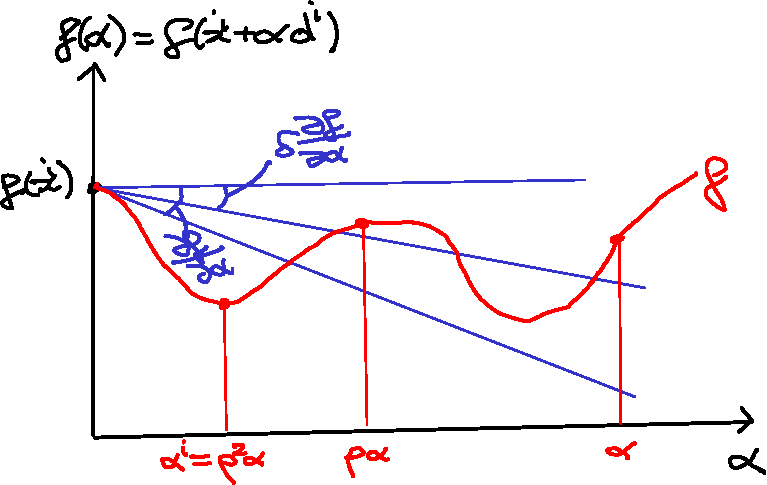
\includegraphics[width=0.7\textwidth]{line_search_backtrack-crop.pdf} 
\end{frame}

%%%%%%%%%%%%%%%%%%%%%%%%%%%%%%%%%%%%%%%%%%%%%%%%%%%%%%%%%%%%%%%%%%
\begin{frame}
\frametitle{Approximate line search (3)} 
At iteration $i$:
\begin{block}{Backtracking line search (Armijo)}
\begin{algorithmic}
\REQUIRE $d^i$ a descent direction, $x^i$, $\delta \in [0,1]$, $\rho \in ]0,1[$, $C>0$
\STATE (defaults: $\delta=0.1,~\rho=0.5,~C=1$)
\STATE initialize step size: $\alpha = \max(C \times \lVert \grad f(x^i) \rVert ~,~ \sqrt{n}/100) $ 
\WHILE{$f(x^i + \alpha d^i) \ge f(x^i) + \delta \alpha \grad f(x^i)^\top  d^i$}
\STATE decrease step size: $\alpha \leftarrow \rho \times \alpha$
\ENDWHILE 
\RETURN $\alpha^i \leftarrow \alpha$
\end{algorithmic}
\end{block}
From now on, use line search, and the number of calls to $f$ is no longer equal to the iteration number since many function calls can be done during a line search within a single iteration.
\end{frame}

%%%%%%%%%%%%%%%%%%%%%%%%%%%%%%%%%%%%%%%%%%%%%%%%%%%%%%%%%%%%%%%%%%
\begin{frame}
\frametitle{Approximate line search (4)} 
Look at what line search does to $f(x)=$ Rosenbrock where fixed step size diverged
\begin{center}
\begin{minipage}[b]{0.3\textwidth}
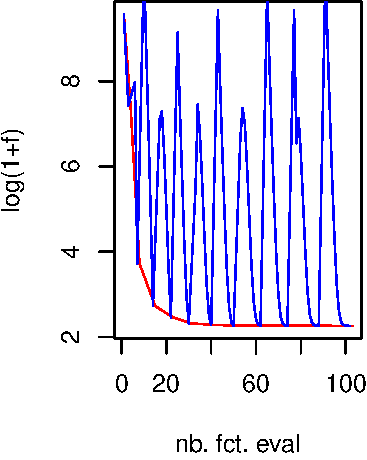
\includegraphics[width=\textwidth]{gradient_rosen_LS_f-crop.pdf} 
\end{minipage}
\hspace{1.cm}
\begin{minipage}[b]{0.3\textwidth}
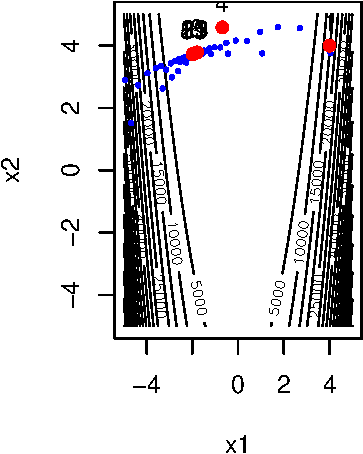
\includegraphics[width=\textwidth]{gradient_rosen_LS_x-crop.pdf} 
\end{minipage}
\end{center}
Better, but not perfect: oscillations make progress very slow.
\end{frame}

%%%%%%%%%%%%%%%%%%%%%%%%%%%%%%%%%%%%%%%%%%%%%%%%%%%%%%%%%%%%%%%%%%
\begin{frame}
\frametitle{Gradient convergence speed} 
$f(x) = \frac{1}{2} x^\top H x$ in $n=10$ dimensions, $H>0$, not aligned with the axes, condition number = 10.
\begin{center}
\mbox{
\begin{minipage}[c]{0.37\textwidth}
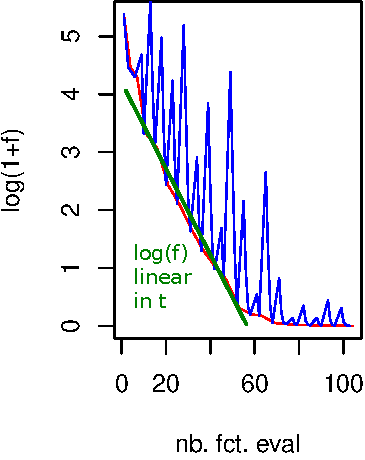
\includegraphics[width=\textwidth,height=6cm]{gradient_quad_d10_cond10_LS-lin-crop.pdf} 
\end{minipage}
\hspace{0.5cm}
\begin{minipage}[c]{0.57\textwidth}
Empirically (for proofs and more info cf. \cite{ravikumar17}): on convex and differentiable functions, gradient search with line search progresses at a speed such that
$f(x^t) \propto \xi \gamma^t$ where $\gamma \in [0,1[$. 
Equivalently, to achieve $f(x^t) < \varepsilon$, $t>\mathcal O(\log(1/\varepsilon))$
\vskip\baselineskip
{\scriptsize
$\log f(x^t) \propto t \log(\gamma) + \log(\xi) ~\Rightarrow~\log(\gamma)<0$ slope of the green curve.\\
$\xi \gamma^t < \varepsilon \Leftrightarrow t > \frac{\log(\varepsilon) - \log(\xi)}{\log(\gamma)} = \frac{-1}{\log(\gamma)}\log(\xi/\varepsilon)$\\ $\Rightarrow~ t>\mathcal O(\log(1/\varepsilon))$ .
}% end scriptsize
\end{minipage}
} % end mbox
\end{center}
\end{frame}


%%%%%%%%%%%%%%%%%%%%%%%%%%%%%%%%%%%%%%%%%%%%%%%%%%%%%%%%%%%%%%%%%%
\begin{frame}
\frametitle{Gradient descent oscillations} 
Perfect line search solves
\begin{equation*}
\alpha^i = \arg\min_{\alpha>0} f(\alpha) ~\text{ where }~ f(\alpha) = f(x^i+\alpha d^i) 
\end{equation*}
Necessary conditions of optimal step size: 
\begin{equation*}
\frac{df(\alpha^i)}{d\alpha} = \sum_{j=1}^n \frac{\partial f(x^i + \alpha^i d^i)}{\partial x_j} \frac{\partial x_j}{\partial \alpha}
= \grad f(x^{i+1})^\top . d^i = 0
\end{equation*}
If the direction is the gradient, 
\begin{equation*}
{-d^{i+1}}^\top . d^i = 0 ~\text{ i.e. } d^{i+1} \text{ and } d^i \text{ perpendicular}
\end{equation*}
\begin{center}
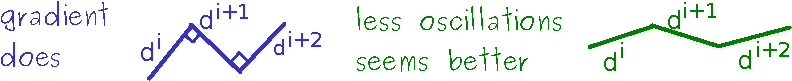
\includegraphics[width=\textwidth]{oscillations-crop.pdf} 
\end{center}
\end{frame}


\section{Improved gradient based searches}

%%%%%%%%%%%%%%%%%%%%%%%%%%%%%%%%%%%%%%%%%%%%%%%%%%%%%%%%%%%%%%%%%%
\begin{frame}%[allowframebreaks]
\frametitle{Course outline} 
\begin{multicols}{2}
\begin{center} \textbf{An introduction to optimization for machine learning} \end{center}
\tableofcontents[currentsection]
\end{multicols}
\end{frame}

\subsection{Search directions for acceleration}

%%%%%%%%%%%%%%%%%%%%%%%%%%%%%%%%%%%%%%%%%%%%%%%%%%%%%%%%%%%%%%%%%%
\begin{frame}
\frametitle{Gradient with momentum (1)} 
Recall fixed step gradient descent, 
\begin{equation*} 
%x^{i+1} = x^i + \alpha s^i  \quad\text{ where }\quad s^i= -\grad f(x^i) 
x^{i+1}= x^i - \bar\alpha \grad f(x^i) \quad\text{ i.e., }\quad s^i = x^{i+1}-x^i = - \bar\alpha \grad f(x^i)
\end{equation*} 
$s^i$, the step, eventually corrected by a line search ($x^{i+1}= x^i + \alpha^i s^i/\lVert s^i \rVert$).
Introduce a momentum (a memory) in the search step \cite{polyak1964some},
\begin{equation*} 
s^i = -\bar\alpha\grad f(x^i) + \beta (x^i -x^{i-1})
\end{equation*} 
where\footnote{alternatively, for iteration varying momentum, $\beta^i=(i-2)/(i+1)$} $\beta = 0.9$.\\
\vspace{-0.2cm}
\begin{minipage}[c]{0.5\textwidth}
This should contribute to avoid the oscillations occuring at the botton of valleys.\\
$s^i$ still a descent direction (assuming perfect line search).
\end{minipage}
\begin{minipage}[c]{0.4\textwidth}
\begin{center}
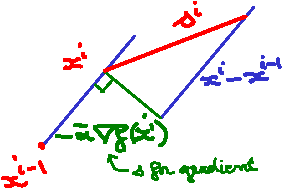
\includegraphics[width=0.9\textwidth]{momentum-crop.pdf} 
\end{center}
\end{minipage}
\end{frame}

%%%%%%%%%%%%%%%%%%%%%%%%%%%%%%%%%%%%%%%%%%%%%%%%%%%%%%%%%%%%%%%%%%
\begin{frame}
\frametitle{Gradient with momentum (2)} 
%Back to Rosenbrock, $d=2$, $x^\star = (1,1) ~,~ f(x^\star) = 0$,\\ 
%budget=4000, $x^1=(4,4)$
%\vspace{-0.3cm}
%\begin{center}
%\begin{minipage}[c]{0.35\textwidth}
%\begin{center}
%gradient\\
%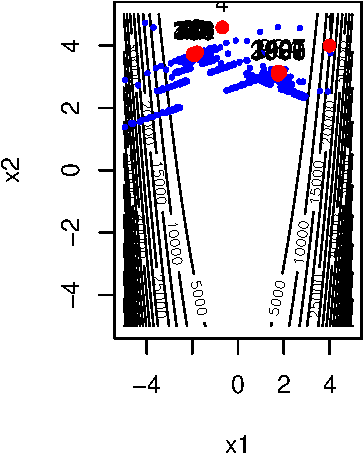
\includegraphics[width=\textwidth]{gradient_rosen_LS_budg4000_x-crop.pdf} 
%\end{center}
%\end{minipage}
%\begin{minipage}[c]{0.35\textwidth}
%\begin{center}
%momentum\\
%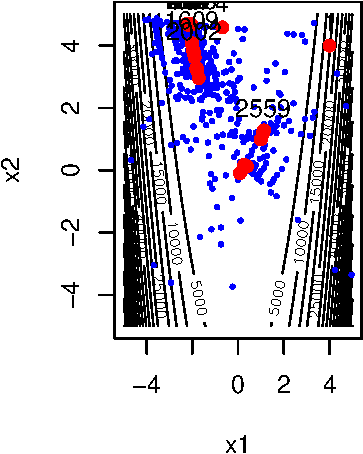
\includegraphics[width=\textwidth]{momentum_rosen_LS_budg4000_x-crop.pdf} 
%\end{center}
%\end{minipage}
%\end{center}
%The momentum acceleration allows to find the solution.
Quadratic function, 10D, condition number = 300, starts from [4,\ldots,4]
\begin{center}
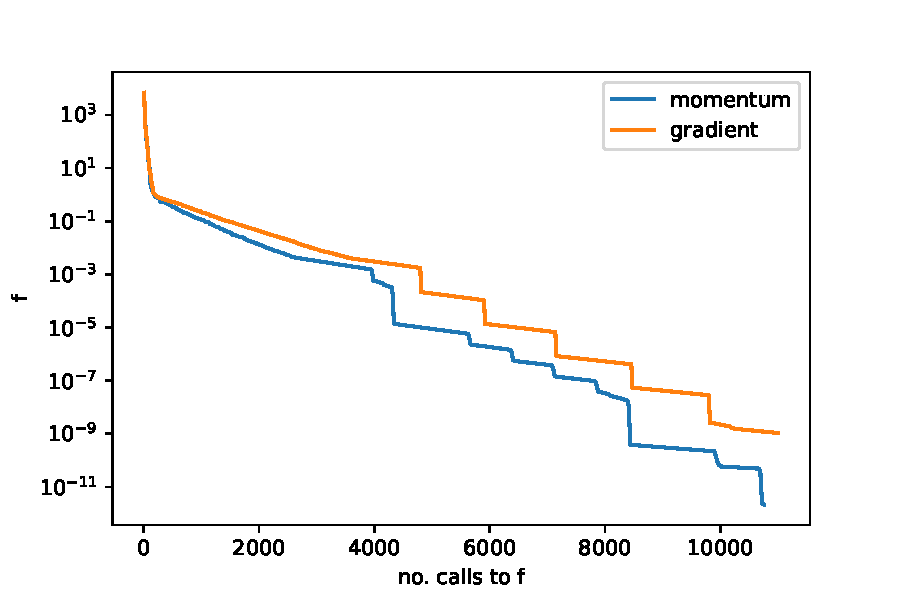
\includegraphics[width=0.7\textwidth]{grad_momentum_quad_10D.pdf} 
\end{center}
The momentum acceleration gains 3 order of magnitudes in this steep valley.
\end{frame}

%%%%%%%%%%%%%%%%%%%%%%%%%%%%%%%%%%%%%%%%%%%%%%%%%%%%%%%%%%%%%%%%%%
\begin{frame}
\frametitle{Nesterov accelerated gradient (NAG)} 
Same idea as the momentum direction, but anticipate the position of the next point in the gradient calculation
\cite{nesterov1983method}:
\begin{equation*} 
s^i = -\bar\alpha \grad f(x^i+\beta (x^i-x^{i-1})) + \beta (x^i -x^{i-1})
\end{equation*} 
\begin{minipage}[c]{0.5\textwidth}
On the sketch, $\grad f$ turns upwards and the step is adjusted accordingly.\\
$s^i$ is no longer necessarily a descent direction.
\end{minipage}
\begin{minipage}[c]{0.4\textwidth}
\begin{center}
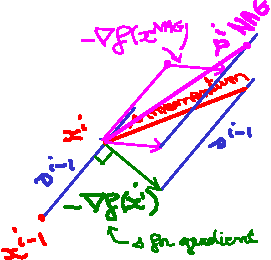
\includegraphics[width=0.9\textwidth]{nag-crop.pdf} 
\end{center}
\end{minipage}
\end{frame}

%%%%%%%%%%%%%%%%%%%%%%%%%%%%%%%%%%%%%%%%%%%%%%%%%%%%%%%%%%%%%%%%%%
\begin{frame}
\frametitle{Comparison of methods (1)} 
Rosenbrock, $d=2$: ability to handle curved ravines
\begin{center}
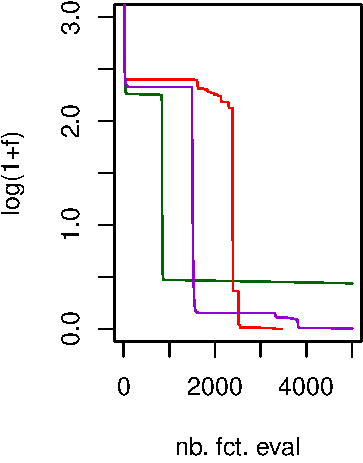
\includegraphics[width=0.4\textwidth]{rosen_comparison-crop.pdf} \\
green=gradient, red=momentum, violet=NAG
\end{center}
\end{frame}

%%%%%%%%%%%%%%%%%%%%%%%%%%%%%%%%%%%%%%%%%%%%%%%%%%%%%%%%%%%%%%%%%%
\begin{frame}
\frametitle{Comparison of methods (2)} 
Test convergence speed on quadratic function, $d=10$, cond. nb. = 100.
{\small green=gradient, red=momentum, violet=NAG}
\\\vskip\baselineskip
\begin{minipage}[c]{0.4\textwidth}
\begin{center}
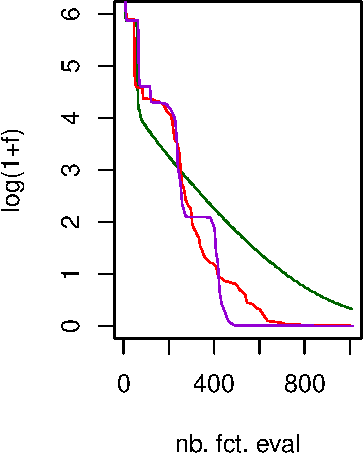
\includegraphics[width=\textwidth]{quadratic_d10_cond100_comparison-crop.pdf} 
\end{center}
\end{minipage}
\hspace{0.6cm}
\begin{minipage}[c]{0.4\textwidth}
In accordance with theory, convergence speed of NAG is better than momentum which is better than gradient.\\
Note however the plateaus (or ``ripples'') typical of NAG and likely magnified by the finite difference
approximation to the gradient.
\end{minipage}
\end{frame}

% a word on convergence of momentum and nag: linear, just the constant changes, which is a lot
% compare curves

\subsection{A word about constraints}

%%%%%%%%%%%%%%%%%%%%%%%%%%%%%%%%%%%%%%%%%%%%%%%%%%%%%%%%%%%%%%%%%%
\begin{frame}%[allowframebreaks]
\frametitle{Course outline} 
\begin{multicols}{2}
\begin{center} \textbf{An introduction to optimization for machine learning} \end{center}
\tableofcontents[currentsection]
\end{multicols}
\end{frame}

%%%%%%%%%%%%%%%%%%%%%%%%%%%%%%%%%%%%%%%%%%%%%%%%%%%%%%%%%%%%%%%%%%
\begin{frame}
\frametitle{A word about constraints} 
\begin{equation*}
\left\{
\begin{array}{l}
\min_{x \in \mathcal S} f(x) \quad,\quad \mathcal S = \Rset[n]\\
\text{such that  } g_i(x) \le 0 \quad , \quad i=1,m
\end{array}
\right.
\end{equation*}
\end{frame}

%%%%%%%%%%%%%%%%%%%%%%%%%%%%%%%%%%%%%%%%%%%%%%%%%%%%%%%%%%%%%%%%%%
\begin{frame}
\frametitle{Bound constraints} 
$\mathcal S$ is an hypercube of $\Rset[n]$, $\mathcal S = [LB,UB] \subset \Rset[n]$.
\vskip\baselineskip
It could be described by constraints, 
$g_{2i-1}(x) \coloneqq LB_i - x_i \le 0$,
$g_{2i}(x) \coloneqq x_i - UB_i \le 0$, $i=1,\ldots,d$
but these constraints are so simple that they can be directly handled by projection.\\
\mbox{
\begin{minipage}[c]{0.4\textwidth}
If $x^i$ is at a bound and the search direction $d^i$ takes it outside$^a$
$\mathcal S = [LB,UB]$, 
project the search direction vector onto the active bound.\\
Exercise: how to code this?
\end{minipage}
\hspace{0.7cm}
\begin{minipage}[c]{0.4\textwidth}
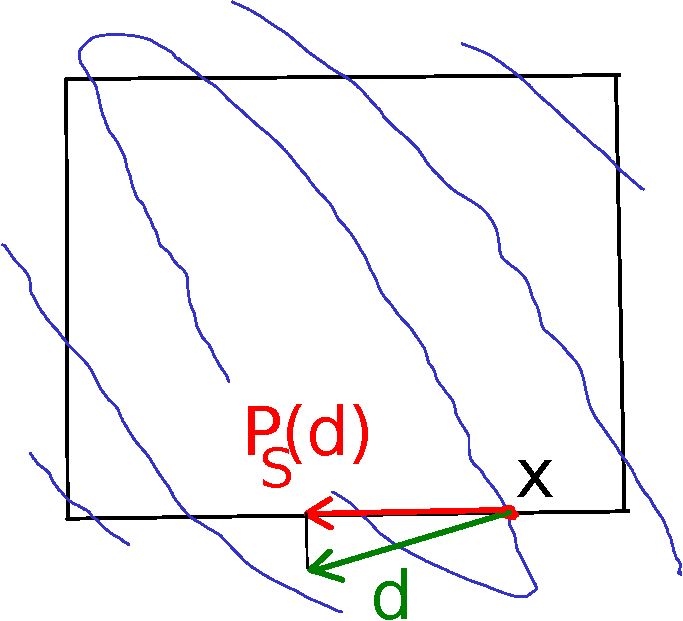
\includegraphics[width=\textwidth]{proj_bound-crop.pdf}
\end{minipage}
}
\\
{$^a$\small This can even happen for a convex function in a convex $\mathcal S$, as the drawing shows.} 
\end{frame}


%%%%%%%%%%%%%%%%%%%%%%%%%%%%%%%%%%%%%%%%%%%%%%%%%%%%%%%%%%%%%%%%%%
\begin{frame}
\frametitle{Constraints handling by penalizations (1)} 
\vspace{-0.5cm}
\begin{equation*}
\left\{
\begin{array}{l}
\min_{x \in \mathcal S \in \Rset[d]} f(x) \\
\text{such that  } g(x) \le 0 
\end{array}
\right.
\end{equation*}
\hfill{\scriptsize (vector notation for the constraints)}\\
We give two techniques to aggregate $f$ and the $g_i$'s into a new objective function 
(to minimize).
\vskip\baselineskip
\textbf{External penalty function}: penalize points that do not satisfy the constraints
\begin{equation*}
f_r(x) = f(x) + r \left[\max(0,g(x)) \right]^2 \quad,\quad r>0 
\end{equation*}
\vspace{-0.5cm}
\begin{itemize}
\item{Pros}: simple, $\grad f_r()$ continuous accross the constraint boundary (if $f$ and $g$ are)
\item{Cons}: Convergence by the infeasible domain (hence external), need to find $r$ large enough to reduce infeasibility, but not too large because of numerical issue (high curvature accross constraint)
\end{itemize}
\end{frame}

%%%%%%%%%%%%%%%%%%%%%%%%%%%%%%%%%%%%%%%%%%%%%%%%%%%%%%%%%%%%%%%%%%
\begin{frame}
\frametitle{Constraints handling by penalizations (2)} 
\textbf{Lagrangian}: for problems without duality gap\footnote{cf. duality, out of scope for this course}, e.g., convex problems, there exists Lagrange multipliers $\lambda^\star$ such that 
\begin{equation*}
\begin{split}
& x^\star \in \arg \min_{x \in \mathcal S} L(x;\lambda^\star) \\
&\text{where } L(x;\lambda^\star) \coloneqq f(x) + \lambda^\star g(x)
\end{split}
\end{equation*}
The Lagrangian $L(;\lambda^\star)$ is (when no duality gap) a valid penalty function.
\begin{itemize}
\item{Pros}: duality provides a way to calculate $\lambda^\star$, yields a feasible solution.
\item{Cons}: estimating $\lambda^\star$ has a numerical cost. 
For most problems with local optima there is a duality gap $\Rightarrow$ rely on augmented Lagrangians$^4$.
\end{itemize}
\end{frame}

%%%%%%%%%%%%%%%%%%%%%%%%%%%%%%%%%%%%%%%%%%%%%%%%%%%%%%%%%%%%%%%%%%
\begin{frame}
\frametitle{Constraints handling by penalizations (3)} 
Example: $f(x)=(x-2)^2$, $g(x)=4-x\le 0$, $x^*=4$, convex problem
\vskip\baselineskip
\mbox{
\begin{minipage}[c]{0.35\textwidth}
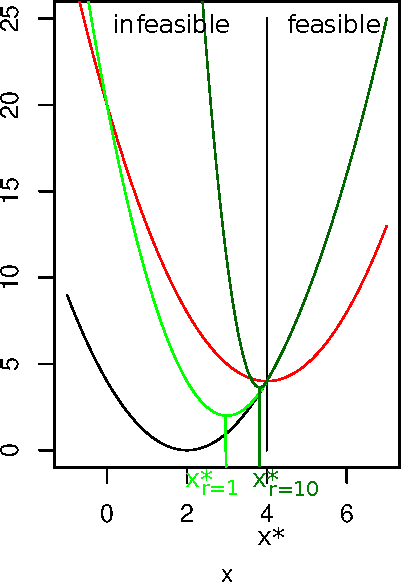
\includegraphics[width=\textwidth]{constraints_methods_annoted-crop.pdf}
\end{minipage}
\hspace{0.5cm}
\begin{minipage}[c]{0.6\textwidth}
$f$ and $g$ in black, $L(x;\lambda^\star=4)$ in red, 
exterior penalty $f_r()$ with $r=1$ and 10 in light and dark green, respectively.
\vskip\baselineskip
The Lagrangian is a valid penalty here. 
\vskip\baselineskip
As $r$ grows, $x_r^\star \rightarrow x^\star$ but the curvature of $f_r()$ increases.
\end{minipage}
}
\end{frame}

%%%%%%%%%%%%%%%%%%%%%%%%%%%%%%%%%%%%%%%%%%%%%%%%%%%%%%%%%%%%%%%%%%
\begin{frame}
\frametitle{Comments on gradient based descent algorithms} 
\begin{minipage}[c]{0.5\textwidth}
Use on nondifferentiable functions: theoretically may converge at a point which is not a minimum even on convex functions (e.g., if an iterate is at a kink). This rarely happens in practice. 
Try function $f(x) = \sum_{i=1}^n \lvert x_i \rvert$ (``L1norm'') with the code. 
\end{minipage}
\begin{minipage}[c]{0.4\textwidth}
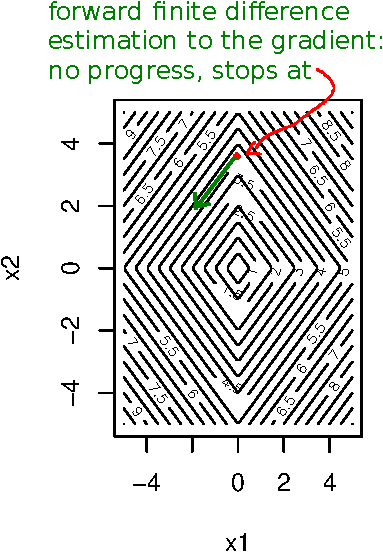
\includegraphics[width=\textwidth]{L1norm_contour-premconv-crop.pdf} 
\end{minipage}
\\
Main flaw: gets trapped in local minima.
\end{frame}

\subsection{Making it more global: restarts}

%%%%%%%%%%%%%%%%%%%%%%%%%%%%%%%%%%%%%%%%%%%%%%%%%%%%%%%%%%%%%%%%%%
\begin{frame}
\frametitle{Restarted local searches} 
Simple principle: restart descent searches from initial points chosen at random.\\
Use randomness to make deterministic descent searches more robust.\\
A mix between 2 extremes: local vs global, line search vs volume search, specific (to unimodal differentiable 
functions) vs without assumption, efficient vs very slow.\\
Simplistic implementation (cf. code provided) \\
\hspace{5cm} at a cost $\times$ \texttt{nb\_restarts}:
\vspace{-0.4cm}
\begin{center}
\begin{minipage}[t]{\textwidth}
\begin{algorithmic}
\REQUIRE \texttt{budget}, \texttt{nb\_restarts}
\FOR {\texttt{i in 1} \TO \texttt{nb\_restarts} }
\STATE \texttt{xinit <- runif(n=d,min=LB,max=UB)}
\STATE \texttt{res<-gradient\_descent(xinit,budget=budget/nb\_restarts)}
\STATE {update global search results}
\ENDFOR
\end{algorithmic}
\end{minipage}
\end{center}
\end{frame}

%%%%%%%%%%%%%%%%%%%%%%%%%%%%%%%%%%%%%%%%%%%%%%%%%%%%%%%%%%%%%%%%%%
\begin{frame}
\frametitle{Restarted local searches: example} 
Execution of the \texttt{restarted\_descent} file. \\
\texttt{fun <-rastrigin, d<-2, budget<-1000, nb\_restart<-10}:
\begin{center}
\mbox{
\begin{minipage}[t]{0.4\textwidth}
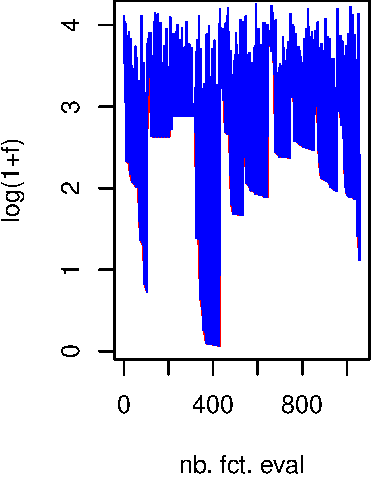
\includegraphics[width=\textwidth]{rastrigin_budget1000_restart10_f-crop.pdf}
\end{minipage}
\vspace{0.7cm}
\begin{minipage}[t]{0.4\textwidth}
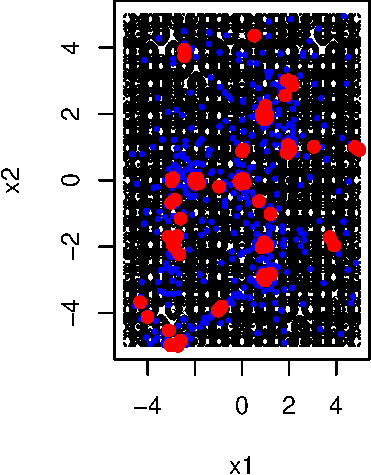
\includegraphics[width=\textwidth]{rastrigin_budget1000_restart10_x-crop.pdf}
\end{minipage}
}
\end{center}
\end{frame}


\section{Application to neural network}

%%%%%%%%%%%%%%%%%%%%%%%%%%%%%%%%%%%%%%%%%%%%%%%%%%%%%%%%%%%%%%%%%%
\begin{frame}%[allowframebreaks]
\frametitle{Application to neural network} 
\begin{center}
The practical applications are available through the \texttt{project} notebook on github,
cf. \url{https://github.com/rleriche/Optimization_AI_Cotonou_2022/blob/main/Code/project.ipynb}
\end{center}
\end{frame}

\section*{Conclusions}

%%%%%%%%%%%%%%%%%%%%%%%%%%%%%%%%%%%%%%%%%%%%%%%%%%%%%%%%%%%%%%%%%
\begin{frame}
\frametitle{Conclusions}
\begin{itemize}
\item Numerical optimization is a fundamental technique for quantitative decision making, statistical modeling, machine learning, \ldots
\item The enthousiasm for machine learning has led to very many optimization algorithms which we did not discuss in this introductory course: see for example \cite{sun2019survey,sra2012optimization}. 
\item Also not covered yet emerging: Bayesian optimization for hyper-parameters tuning (regularization constants, number of NN layers, types of neurons, parameters of the gradient based algorithms) \cite{snoek2012practical}.
\end{itemize}
\end{frame}

\section{Bibliography}

%=======================================================================================
\begin{frame}[allowframebreaks]
\frametitle{References}
\scriptsize
%\vspace{-1.cm}
%\setbeamertemplate{bibliography item}{[\theenumiv]} % to have numbers in biblio with beamer
%   \bibliographystyle{plain}
   \bibliographystyle{apalike}
   \bibliography{biblio}
\end{frame}

\end{document}
